
\documentclass[12pt,a4]{article}
\author{Yujie Lu \quad Jiabao Ji \quad Tong Chen}
\newcommand{\handoutdate}{2020-03-05}
\newcommand{\firstduedate}{2020-03-10}
\newcommand{\finalduedate}{2020-03-17 before class}
\usepackage{pythonhighlight}
\usepackage{import}
\usepackage[many]{tcolorbox}
\tcbuselibrary{skins, breakable, theorems}
\tcolorboxenvironment{exercise}{
  enhanced,
  borderline={0.4pt}{0.4pt}{black},
  boxrule=0.4pt,
  colback=white,
  coltitle=black,
  sharp corners,
}




\usepackage{graphicx,amsmath,amssymb,amsthm, boxedminipage}



\usepackage{algorithm}
\usepackage{algpseudocode}


\newtheorem{theorem}{Theorem}%[section]
\newtheorem{proposition}[theorem]{Proposition}
\newtheorem{lemma}[theorem]{Lemma}
\newtheorem{corollary}[theorem]{Corollary}
\newtheorem{definition}[theorem]{Definition}



\newcommand{\scalar}[2]{\ensuremath{\langle #1, #2\rangle}}
\newcommand{\floor}[1]{\left\lfloor #1 \right\rfloor}
\newcommand{\ceil}[1]{\left\lceil #1 \right\rceil}
\newcommand{\norm}[1]{\|#1\|}
\newcommand{\pfrac}[2]{\left(\frac{#1}{#2}\right)}
\newcommand{\nth}[1]{#1\textsuperscript{th}}

% \newcommand{\nth}[1]{#1\textsuperscript{th}}
\newcommand{\E}{\mathop{\mathbb{E\/}}}
\newcommand{\N}{\mathbb{N}}

\newcommand{\R}{\mathbb{R}}

\newtheorem{exercise}[theorem]{Exercise}
\newtheorem{exerciseD}[theorem]{*Exercise}
\newtheorem{exerciseDD}[theorem]{**Exercise}

\let\oldexercise\exercise
\renewcommand{\exercise}{\oldexercise\normalfont}

\let\oldexerciseD\exerciseD
\renewcommand{\exerciseD}{\oldexerciseD\normalfont}

\let\oldexerciseDD\exerciseDD
\renewcommand{\exerciseDD}{\oldexerciseDD\normalfont}


 
\begin{document}

\date{}

\title{CS 217 -- Algorithm Design and Analysis \\ 
  \vspace{3mm}
{\large	Shanghai Jiaotong University, Fall 2019\\
}
}
\maketitle

\noindent
Handed out on \handoutdate{}\\
First submission and questions due on \firstduedate{}\\
You will receive feedback from the TA.\\
Final submission due on \finalduedate{}


\section{Bit Complexity, Recursion, and Dynamic Programming}

\subsection{Bit Complexity of Euclid's Algorithm}

We have proved that Euclid's algorithm for computing $\gcd(a,b)$ makes at most
$O(\log a)$ iterations. What is the overall running time? Each iteration computes
$u \mod v$ for some integers. This can be done by integer division. What is its running time?
There are very sophisticated algorithms, but python probably does not come with them. 
Recall the ``school method'' for dividing integers. Have a look at the pdf slides on the 
webpage for an illustration of the school method. It is especially simple if we are dealing
with binary numbers. If $a$ and $b$ have at most $n$ bits, then the school method 
has complexity $O(n^2)$.
\begin{exercise}
  Show the following, more precise bound of the school method for integer division:
  If $a$ has $n$ bits and $b$ has $k$ bits, then the school method can be implemented
  to run in $O( k(n-k))$ operations.
\end{exercise}
\begin{proof}
First, we know $n > k$ since $a > b$. To get r, $r = a \% b, (0 \leq r < b)$,
so the bits of $r$, we write it as $b_r$. $b_r < k$.

Remind the procedure of brute-force algorithm of $a \% b$, in each iteration,
$n$ decreases(since we can drop the higher bits). In the final iteration, $n < k$,
also this $n$ is exactly $b_r$, so we don't need to do the iteration $n$ times,
but only $n - k + 1$ times. And each iteration costs $k$ subtraction operation, which is an integer operation,
in all we do no more than $k(n - k+ 1)$ times of basic operations. That is 
$O\left( k\left( n-k \right)  \right) $ basic operations.
\end{proof}
\begin{exercise}
  Show that the bit complexity of Euclid's algorithm, using the school method
  to compute $a \mod b$, is $O(n^2)$. That is,
  if $a$ and $b$ have at most $n$ bits, then $\gcd(a,b)$ makes $O(n^2)$ bit operations.\\
  
  In order to do so, here is python code of the Euclidean algorithm:
\begin{verbatim}
  def euclid(a,b):
    while (b > 0):
        r = a % b # so a = bu+r
        if (r == 0):
            return b
        s = b % r # so b = rv + s
        a = r
        b = s
    return a
\end{verbatim}
Don't be afraid to introduce notation! I recommend to let $n$ denote the number of bits of $a$.
Take some other letters for the number of bits in $b$ and so on.
\end{exercise}
\begin{proof}
		Assume that $\gcd\left( a,b \right) $ takes $t$ iterations and $t \le  2n$. To better represent our ideas.  Let's introduce
		some notations. Conside a process of iterations as follows:
		\[
				\gcd\left( a,b \right) = \gcd\left( x_{t},x_{t-1} \right) \to 
				\gcd\left( x_{t-1},x_{t-2} \right) \to \ldots \to \gcd\left( x_1,0 \right) 
		.\] 
		And $\forall 1\le k\le t$ let $x_{k}$ has $y_{k}$ bits. We know $y_{t}\le n$ plus $x_{k}>x_{k-1}$.
		Hence $\forall k, y_{k}\ge y_{k-1}$.

		Let the operations of all iterations be $T$. And the operations of  $k$th iteration be $T_{k}$. 
		Now apply the conclusion of Exercise 1, we have
		\begin{align*}
				T &= \sum_{k=1}^{t} T_{k} \\
				  &\le \lambda \sum_{k=1}^{t} y_{k}\left( y_{k}-y_{k-1} \right) \\ 
				& \le \frac{\lambda}{2}\left( \sum_{k=1}^{t} \left( y_{k}-y_{k-1} \right)^2 + y_t^2 \right) \\
				  & \le  \frac{\lambda}{2} \left( \sum_{k=1}^{t} \left( y_{k}-y_{k-1} \right)  \right)^2+ \frac{\lambda}{2} y_{t}^2\\
				  & \le  \frac{\lambda}{2} n^2
		.\end{align*} 
		Hence $\gcd\left( a,b \right) $ makes $O\left( n^2 \right) $ operations.
\end{proof}
\subsection{Computing the Binomial Coefficient}

Next, we will investigate the binomial coefficient ${n \choose k}$, which 
you might also know by the notation $C^k_n$. The number ${n \choose k}$ is defined
as the number of subsets of $\{1,\dots,n\}$ which have size exactly $k$. 
This immediately shows that ${n \choose k}$ is $0$ if $k$ is negative or larger than $n$.
You might have seen the following recurrence:
\begin{align*}
 {n \choose k} & = {n-1 \choose k-1} + {n-1 \choose k} \textnormal{ if } n,k \geq 0 \ .
\end{align*}

\begin{exercise}[A Recursive Algorithm for the Binomial Coefficient]
  Using pseudocode, write a recursive algorithm computing
  ${n \choose k}$. Implement it in python! What is 
  the running time of your algorithm, in terms of $n$ and $k$? Would you say it is an efficient
  algorithm? Why or why not?
\end{exercise}
\begin{proof}
recursive code: 
\begin{python}
def recursiveCompute(n, k):
    if (n <= k or k == 0):
        return 1
    else:
        return recursiveCompute(n - 1, k - 1) + recursiveCompute(n - 1, k)
\end{python}

Like recursive algorithm for computing Fib(n), we can get a recursive tree, 
which has $ \binom n k$ leaves and $ \left(2 \binom n k - 1\right) $ nodes in all. 
We can prove it by induction.

Firstly, prove it for a fixed n, to do that, we use an induction. 
And suppose the equation is true for all $m < n$ (base $n = 1$ is trivial).\\
\textbf{Base:} $k = 0:$

Obviously, the recursive tree only has 1 node, which satisfies the equation.\\
\textbf{Induction:} 

To compute $\binom n {k+1} $, we will add a node for $\binom n {k+1}$ as the new root,
and two sub recursive tree for computing $\binom {n - 1} {k}, \binom {n - 1}{k + 1}$, 
whose nodes size is known by induction hypothesis.
The new tree has 
\[
\binom {n-1} {k} + \binom{n - 1} {k + 1} = \binom{n}{k + 1}
.\] 
leaves, and
\[
\left(2\binom{n - 1}{k} - 1 \right)+ \left(2\binom{n - 1}{k + 1} -1\right) + 1
= 2\binom n {k + 1} - 1 
.\] 
nodes.

Similar to the induction above, we can tell for any $n, k$, the result holds.
For the running time analysis, each node in the tree needs to do an addition,
so it's $O\left(2 \binom n k - 1\right)= O\left( \binom{n}{k}  \right) $.
If we consider the cost of addition at each node: $\log \binom{n}{k}$, we get
$O((\binom n k )log(\binom n k))$.

To sum up, the algorithm's time complexity is 
\[ 
		\Omega\left(\binom n k\right)\text{ and } O\left(\binom n k \log\left
		(\binom n k\right)\right).
\]
It's not a good algorithm, since the time complexity is very high, and it does a lot of 
redundant addition.
\end{proof}
\begin{exercise}[A Dynamic Programming Algorithm for the Binomial Coefficient]
  Using pseudocode, write a dynamic programming algorithm
  computing ${n \choose k}$. Implement it in python! What is it running time
  in terms of $n$ and $k$?
  Would you say your algorithm is efficient? Why or why not?
\end{exercise}
\begin{proof}
code:
\begin{python}
def dpCompute(n, k):
    a = [[0 for x in range(k + 1)] for y in range(n + 1)] 
    for i in range (n + 1):
        a[i][0] = 1
        if i <= n - k:
            for j in range (1, min(i, k) + 1):
                a[i][j] = a[i - 1][j - 1] + a[i - 1][j]
        else:
            for j in range(i - (n - k), min(i, k) + 1):
                a[i][j] = a[i - 1][j - 1] + a[i - 1][j]
    return a[n][k]
\end{python}
The algorithm needs to do $n$ iterations, for iterations $i \le  n - k$, 
we should do $\mathrm{min}  (i, k)$ additions, and for $i > n - k$, we should do $\mathrm{min} (i, k) - i - (n - k)$ additions
(since there is no node of $\binom i j $ if $ i > n - k, j < i - (n - k)$ in the recursive tree)
In all, we need to compute
$$
    \sum_{i = 1}^{n - k} \sum_{j = 1}^{min(i, k)} 1 + 
    \sum_{i = n - k + 1}^{n + 1}\sum_{j = i - (n - k)}^{min(i, k) + 1} 1
    = n (n - k)
$$
additions. 

This is not trivial, so we draw a picture to better visualize this
\begin{figure}[ht]
    \centering
	\incfig[0.8]{triangle}
    \caption{How much do we compute.}
    \label{fig:triangle}
\end{figure}

Consider the cost of each addition, the algorithm is $\Omega(n(n - k))$ and $O(n(n - k) log \binom n k)$.
It's much more efficcient than the recursive algorithm. I think it's efficcient.


\end{proof}

\begin{exercise}[Binomial Coefficient modulo 2]
  Suppose we are only interested in whether ${n \choose k}$ is even or odd,
  i.e., we want to compute ${n \choose k}  \mod 2$. You could do this by computing 
  ${n \choose k}$ using dynamic programming and then taking
  the result modulo $2$. What is the running time? Would you say this algorithm
  is efficient? Why or why not?
\end{exercise}
\begin{proof}
  The running time is similar to Exer.4, but since we only needs to know whether the result modula 2 is 1 or 0,
  we don't need to compute addition at each node but only a bool compute. \\
  \hspace*{1em} So the dynamic algorithm is $\Theta (n(n - k))$.\\
  \hspace*{1em} To this question specifically,not efficcient, 
  we don't have to compute the value of $\binom n k$ at all.\\
  Below is the python code.
  \newpage
  \begin{python}
  def hasNtwoFactor(asking):
      res = 0
      while (asking % 2 == 0):
          res += 1
          asking = asking / 2
      return res
  
  def isEvenOrOdd(n, k):
      numerator = 0
      dominator = 0
      for i in range(1, n + 1):
          numerator += hasNtwoFactor(i)
      for i in range(1, k + 1):
          dominator += hasNtwoFactor(i)
      for i in range(1, n - k + 1):
          dominator += hasNtwoFactor(i)
      if (numerator - dominator > 0):
          return bool(1)
      else:
          return bool(0)
  \end{python}
  it's an $\Theta(n log(n))$ algorithm, faster than dpCompute.
  

We also have another algorithm based on \textbf{Lucas Theorem} 
\begin{python}
def C(n, k):
	if n & k == k:
        return 1;
    else:
        return 0;
\end{python}

Now, let's proof this simple algorithm why it's correct.
\begin{theorem}
	\textbf{(Lucas Theorem)} For non-negative integers \textit{m} and \textit{n} and a prime \textit{p}, the following congruence relation holds:
	$${m \choose n} \equiv \prod_{i=0}^k {m_i \choose n_i} ( mod\ p),$$
	where
	$$m=m_kp^k+m_{k-1}p^{k-1}+\cdots+m_1p+m_0$$,
	and
	$$n=n_kp^k+n_{k-1}p^{k-1}+\cdots+n_1p+n_0$$
	are the base p expansions of m and n respectively. This uses the convention that ${m\choose n}=0$ if $m<n$.
\end{theorem}
Here, we let p = 2, and we have ${0 \choose 0}={1\choose 0}={1 \choose 1}=1$ and ${0 \choose 1}=0$. Hence, we get ${n\choose k}\equiv 1 (mod\ 2)$ if and only if every bit of k is less than that of n in binary representation. That means $n\ and\ k = k$.

The time complexity of this algorithm is $\Theta(log(n))$
\end{proof}
\begin{exercise}
  Remember the ``period'' algorithm for computing $F'_n := (F_n \mod k)$ discussed in class:
  (1) find some $i,j$ between $0$ and $k^2$ for which 
  $F'_{i} =  F'_{j}$ and $F'_{i+1} = F'_{j+1} $. 
  Then for $d := j-i$ the sequence $F'_{n}$ will repeat every $d$ steps, as there will be a cycle.
  This cycle can either be a ``true cycle'' or a ``lasso'':
  \begin{center}
  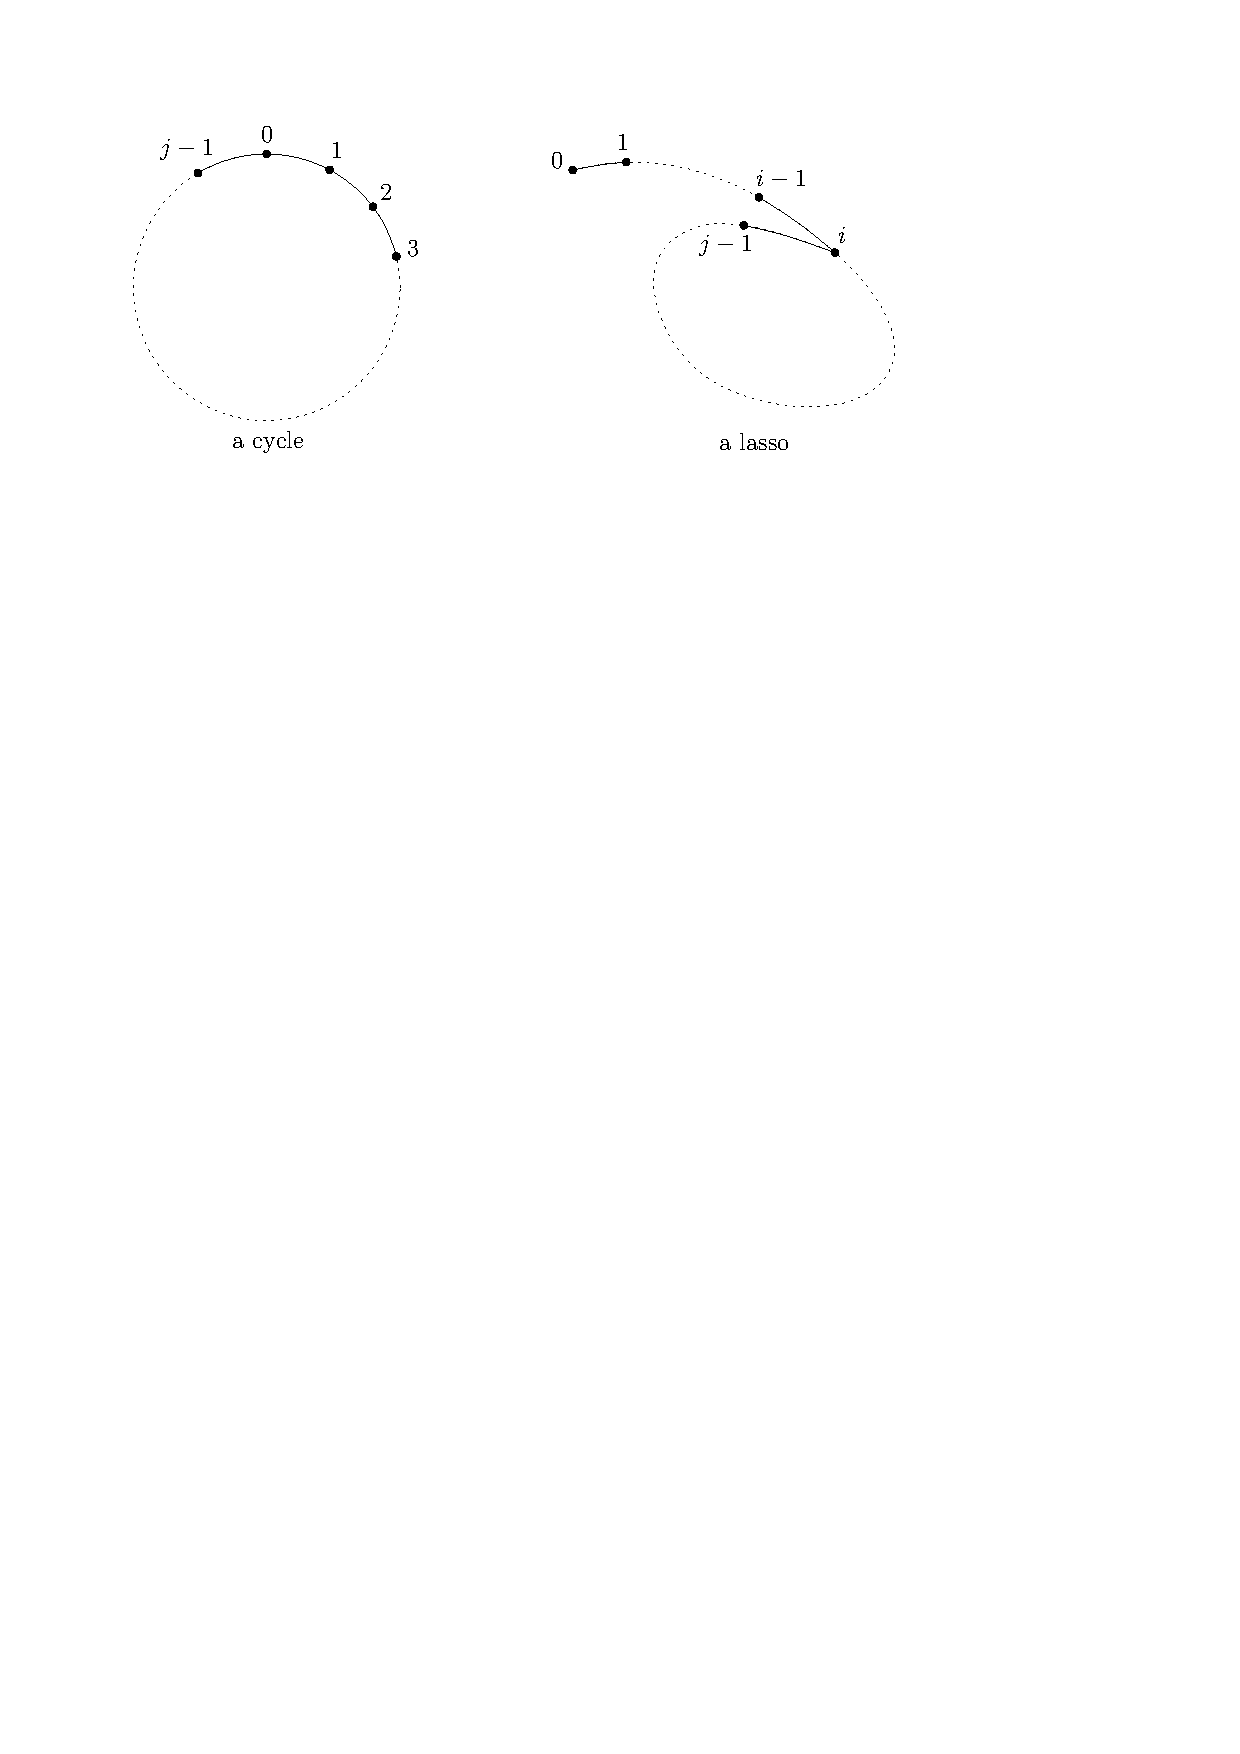
\includegraphics[width=0.8\textwidth]{figures/cycle-and-lasso.pdf}
  \end{center}
  
  Show that a lasso cannot happen. That is, show 
  that the smallest $i$ for which this happens is $0$, i.e, for some $j$ we have
  $F'_0 = F'_j$ and $F'_1 = F'_{j+1}$ and thus $F'_n = F'_{n \textnormal{ mod }  j}$.
\end{exercise}
  
\begin{proof}
		Consider a pair $g\left( i \right) =\left( F'_{i-1},F'_{i} \right) , i\ge 0$. We know that
		$\forall i, g\left( i \right) \in [0,n)\times [0,n)$ which is a finite set with $k^2$ members.

		Consider the following set 
		\[
				A = \{ g\left( 1 \right) ,g\left( 2 \right) ,\ldots, g\left( k^2 \right) , g\left( k^2+1 \right) \} 
		.\] 
		By \textbf{Pigeonhole Principle}, we know that $\exists r< s\in \{1,2,\ldots,k^2+1\} $ such that 
		$g\left( r \right) =g\left( s \right) $ which is
		\[
				F'\left( r-1 \right) = F'\left( s-1 \right) , \quad F'\left( r \right)  = F'\left( s \right) 
		.\] 
		Since $F'\left( r-2 \right)$ is determined by $F'\left( r \right) -F'\left( r-1 \right) $, we can imply that 
		\[
				F'\left( 0 \right)  = F'\left( s-r \right) , \quad F'\left( 1 \right)  = F'\left( s-r+1 \right) 
		.\] 
		Hence this cycle is a ``true cycle".
\end{proof}


\newpage
{\huge\noindent \textbf{Appendix}   \\ \\ } 
{\large Pseudocode for Exercise 3, 4}
\begin{algorithm}[h]
		\caption{A function $f$ using recursive algorithm.}
		\KwIn{input parameters $n,k$}
		\KwOut{$ {n\choose k }$}
		\LinesNumbered
		\If{$n=k$ or $k=0$} {
				return $1$
		} 
		\Else {
				return $f\left( n-1,k-1 \right) + f\left( n-1,k \right) $
		}
\end{algorithm}

\begin{algorithm}[h]
		\caption{A function $g$ using dynamic algorithm.}
		\KwIn{input parameters $n,k$}
		\KwOut{$ {n\choose k }$}
		\LinesNumbered
		a is a 2d array to store results.

		\For{$i$ in  $\{1,2,\ldots,n+1\} $ } {
				a[i][0] = 1
				\If {$i\le n-k $ } {
						\For{$j\le   \mathrm{min}\left( i,k \right) $ }
						{
								update a[i][j]
						}
				} 
				\Else {
						\For {$j \le   \mathrm{min}\left( i,k \right)  \} $} {
								update a[i][j]
						}
				}
		}
		return a[n][k]
\end{algorithm}
\end{document}
